\documentclass[11pt]{article}
\usepackage[utf8]{inputenc}
\usepackage{mathrsfs}
\usepackage{amsmath, amssymb, amsthm, mathtools}
\usepackage{enumitem}
\usepackage{geometry}
\geometry{margin=1in}

% theorem-style environments
\newtheorem{theorem}{Theorem}[section]
\newtheorem{proposition}{Proposition}[section]
\newtheorem{corollary}{Corollary}[section]

\theoremstyle{definition}
\newtheorem{definition}{Definition}[section]
\newtheorem{notationdef}{Notation–Definition}[section]
\newtheorem{example}{Example}[section]
\newtheorem{remark}{Remark}[section]
\newtheorem{application}{Application}[section]
\newtheorem{illustration}{Illustration}[section]
\newtheorem{notation}{Notation}[section]
\newtheorem{properties}{Properties}[section]

\begin{document}
\begin{titlepage}
    \centering
    \vspace*{1cm}
    \rule{\linewidth}{0.5mm} \\[0.4cm]
    { \Huge \bfseries Measure Theory \\[0.2cm] }
    \rule{\linewidth}{0.5mm} \\[3.5cm]
    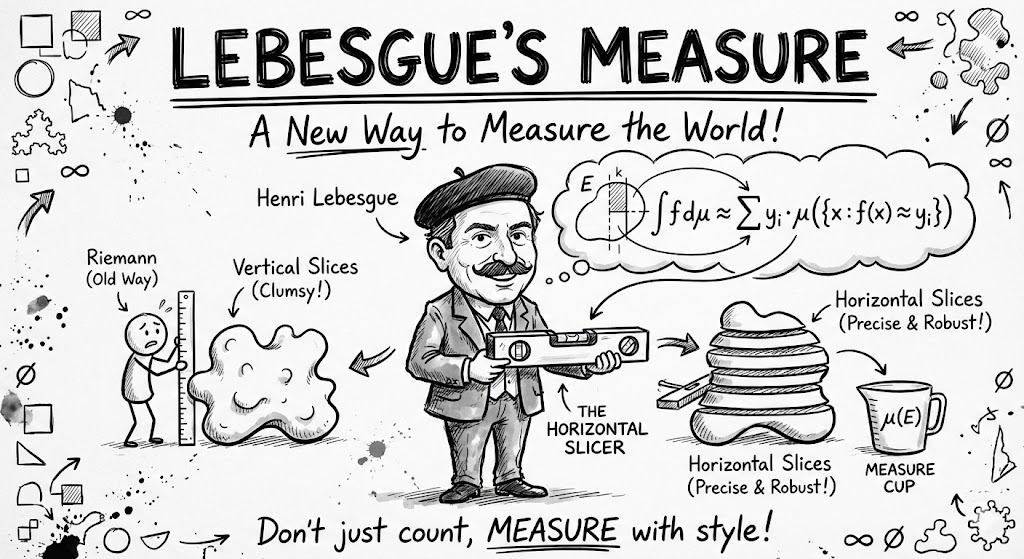
\includegraphics[width=1\linewidth]{figures/cover.jpg}
    \vfill
    \textit{Author:}\\
    {\Large Yuguang XIAO}\\[1cm]
    \today
    \vspace*{1cm}
\end{titlepage}
\newpage
\tableofcontents
\newpage
\section{Elements of the theory of cardinals}
\subsection{Cardinals}
\begin{definition}
Let $X$ and $Y$ be two sets.
We say that $X$ is $\emph{equipotent}$ to $Y$, and we write $X \approx Y$ or $\operatorname{card} X=\operatorname{card} Y$, if there exists a bijection from $X$ onto $Y$.
\end{definition}

It is immediate that every set $X$ is equipotent to itself, because the identity map on $X$ is a bijection from $X$ onto $X$.
If a function $f:X\to Y$ is bijective, then it admits a bijective inverse $f^{-1}:Y\to X$; consequently, if $X\approx Y$, then $Y\approx X$.
Finally, since the composition of two bijections is a bijection, it is clear that if $X\approx Y$ and $Y\approx Z$, then $X\approx Z$.

Thus the relation of equipotence is an equivalence relation on the ``collection of all sets'' whose ``classes'' define the ``cardinals.''
The presence of quotation marks is justified by the fact that the collection of all sets is not itself a set, otherwise that set would be an element of itself.
The naive passage from the equivalence relation of equipotence to the associated equivalence classes is therefore not perfectly satisfactory from the standpoint of rigor.
This obstacle can nonetheless be circumvented, and cardinals can be defined rigorously.

\begin{example}
\begin{enumerate}[leftmargin=2em,label=\arabic*.]
\item $\mathcal P(X)$ and $\{0,1\}^{X}$ are equipotent, because the map
\[
\begin{array}{rcl}
\mathcal P(X) &\longrightarrow& \{0,1\}^{X} \\
A &\longmapsto& \mathbf 1_A
\end{array}
\qquad\text{where}\quad
\mathbf 1_A(x):=\begin{cases}
1,& x\in A,\\[2pt]
0,& x\notin A,
\end{cases}
\]
is bijective.
\item $\mathbb N$ is equipotent to $2\mathbb N$, because $n\mapsto 2n$ is a bijection.
\end{enumerate}
\end{example}


\begin{proposition}
Let $X$ be a set.
The sets $X$ and $\mathcal P(X)$ are not equipotent and, more precisely, there is no surjection from $X$ onto $\mathcal P(X)$.
\end{proposition}

\begin{proof}
Suppose a surjection $f:X\to\mathcal P(X)$ exists.
One could then find a preimage $a\in X$ of the set $A:=\{x\in X : x\notin f(x)\}$, i.e.\ an element $a\in X$ such that $f(a)=A$.
But if $a\in A$ then $a\notin f(a)=A$, and if $a\notin A$ then $a\in f(a)=A$.
Contradiction.
\end{proof}

\begin{notationdef}
\begin{enumerate}[label=(\alph*),leftmargin=2em]
\item If there exists an injection of $X$ into $Y$, we write $\operatorname{card} X \le \operatorname{card} Y$.
\item If $\operatorname{card} X \le \operatorname{card} Y$ and $X,Y$ are not equipotent, we write $\operatorname{card} X < \operatorname{card} Y$.
\end{enumerate}
\end{notationdef}

\begin{theorem}[(Cantor--Bernstein)]
\begin{enumerate}[label=(\alph*),leftmargin=2em]
\item If there exists an injection of $X$ into $Y$, then there exists a surjection from $Y$ onto $X$.
\item If there exists a surjection from $X$ onto $Y$, then there exists an injection of $Y$ into $X$.
\item If there exists an injection (respectively a surjection) of $X$ into $Y$ and an injection (respectively a surjection) of $Y$ into $X$, then $X$ and $Y$ are equipotent; i.e.\ they have the same cardinal.
\item If $X$ and $Y$ are two sets, then exactly one of the following three situations occurs:
\[
\operatorname{card} X < \operatorname{card} Y,\qquad
\operatorname{card} X = \operatorname{card} Y,\qquad
\operatorname{card} X > \operatorname{card} Y .
\]
\end{enumerate}
\end{theorem}

This (difficult) result will be admitted here.

\begin{corollary}
The relation $\le$ is a total order on cardinals.
\end{corollary}

\begin{proof}
Reflexivity is immediate since, for every set $X$, the identity map $Id_X$ is injective.
Antisymmetry follows from point (c).
The composition of two injective maps being injective, the relation $\le$ is clearly transitive.
Totality follows from point (d).
\end{proof}

\begin{illustration}
\begin{enumerate}[label=\arabic*.,leftmargin=2em]
\item If $X\subset Y$, then $\operatorname{card} X\le \operatorname{card} Y$.
\item On the one hand $\operatorname{card}\mathbb N\le \operatorname{card}\mathcal P(\mathbb N)$, because $n\mapsto\{n\}$ is injective;
on the other hand $\operatorname{card}\mathbb N < \operatorname{card}\mathcal P(\mathbb N)$, since by Proposition~1.1 there is no surjection from $\mathbb N$ onto $\mathcal P(\mathbb N)$.
\end{enumerate}
\end{illustration}

\begin{definition}
A set $X$ is infinite if there exists $x_0\in X$ and an injection of $X$ into $X\setminus\{x_0\}$.
Otherwise $X$ is said to be finite and we write $\operatorname{card} X < +\infty$.
\end{definition}

\begin{example}
$\mathbb N$ is infinite, because $n\mapsto n+1$ is an injection from $\mathbb N$ into $\mathbb N\setminus\{0\}$.
\end{example}

\begin{proposition}
If there exists an injection of $X$ into $Y$ and if $X$ is infinite, then $Y$ is infinite.
In particular, as soon as a set contains an infinite subset, the set itself is infinite.
\end{proposition}

\begin{proof}
Let $i$ be an injection of $X$ into $Y$, and let $\varphi$ be an injection of $X$ into $X\setminus\{x_0\}$.
Define $\psi:Y\to Y\setminus\{i(x_0)\}$ by
\[
\psi(y)=
\begin{cases}
y, & \text{if } y\in Y\setminus i(X),\\
i\bigl(\varphi(x)\bigr), & \text{if } y=i(x)\in i(X).
\end{cases}
\]
Then $\psi$ is an injection from $Y$ into $Y\setminus\{i(x_0)\}$.
\end{proof}

\begin{proposition}
A set $X$ is infinite if and only if there exists an injection of $\mathbb N$ into $X$, i.e.\ $\operatorname{card} X \ge \operatorname{card}\mathbb N$.
\end{proposition}

\begin{proof}
Let $X$ be an infinite set.
We show by induction that for every $n\in\mathbb N$ there exist $(n+1)$ distinct elements $x_0,\dots,x_n$ of $X$ and an injection $i_n$ of $X\setminus\{x_0,\dots,x_n\}$ into $X\setminus\{x_0,\dots,x_{n+1}\}$ with $x_{n+1}\in X\setminus\{x_0,\dots,x_n\}$.
The result is true for $n=0$ by the definition of an infinite set.
Assume it true for $n$.
By Proposition~2.2 the set $X\setminus\{x_0,\dots,x_n\}$ is infinite, which yields an injection $j$ from $X\setminus\{x_0,\dots,x_n\}$ into $X\setminus\{x_0,\dots,x_n,x_{n+1}\}$ with $x_{n+1}\in X\setminus\{x_0,\dots,x_n\}$.
Then $i_{n+1}:=j\circ i_n$ is an injection from $X\setminus\{x_0,\dots,x_n\}$ into $X\setminus\{x_0,\dots,x_{n+1}\}$.
Finally, the map $\mathbb N\to X$ given by $n\mapsto x_n$ is injective.

Conversely, the existence of an injection $\mathbb N\to X$ implies that $X$ is infinite by the previous proposition, since $\mathbb N$ is itself infinite.
\end{proof}

\begin{remark}
Proposition~1.3 can be reformulated equivalently as follows:
a set $X$ is finite if and only if $\operatorname{card} X < \operatorname{card}\mathbb N$.
\end{remark}

This expresses the fact that the sets equipotent to $\mathbb N$ are the ``smallest'' infinite sets in the sense of cardinals.

\begin{example}
\begin{enumerate}[leftmargin=2em,label=\arabic*.]
\item $\mathbb R$ is infinite because $\mathbb N\subset\mathbb R$.
\item $\mathcal P(\mathbb N)$ is infinite, since $n\mapsto\{n\}$ is an injection from $\mathbb N$ into $\mathcal P(\mathbb N)$.
However, we already observed that $\operatorname{card}\mathbb N < \operatorname{card}\mathcal P(\mathbb N)$.
Therefore there are several---indeed infinitely many---``classes'' of infinite sets, the smallest of which consists of the sets equipotent to $\mathbb N$.
It is this class that we will now study in more detail.
\end{enumerate}

\end{example}

\subsection{Countable sets}

\begin{definition}
\begin{enumerate}[label=(\alph*),leftmargin=2em]
\item A set $X$ is said to be \emph{countable} if there exists an injection of $X$ into $\mathbb N$, i.e.\ $\operatorname{card} X\le \operatorname{card}\mathbb N$.
\item A set $X$ is said to be \emph{countably infinite} if $X$ is equipotent to $\mathbb N$, i.e.\ $\operatorname{card} X=\operatorname{card}\mathbb N$.
We write $\aleph^0$\,\footnote{$\aleph$ (pronounced ``aleph'') is the first letter of the Hebrew alphabet.} for the countably infinite cardinal.
\item If $\operatorname{card} X > \operatorname{card}\mathbb N$, the set $X$ is said to be \emph{uncountable} (or sometimes \emph{infinitely uncountable}).
\end{enumerate}
\end{definition}

Thus $\mathbb N$ is obviously countably infinite, and $\mathcal P(\mathbb N)$ is uncountable (see the example above).

\begin{remark}
By the Cantor--Bernstein theorem, a set $X$ is countably infinite if and only if it is infinite and countable (which ensures the coherence of the definition).
\end{remark}

We immediately deduce from these definitions the following properties.

\begin{proposition}
\begin{enumerate}[label=(\alph*),leftmargin=2em]
\item A set $X$ is countable if and only if it is finite or countably infinite.
\item Every subset of a countable set is countable.
\item If $X$ is infinite, $Y$ is countable and $X\subset Y$, then $Y$ is countably infinite.
\end{enumerate}
\end{proposition}

\begin{proof}
\emph{(b)} Let $X'\subset X$.
The composite of the canonical injection of $X'$ into $X$ with an injection of $X$ into $\mathbb N$ is an injection of $X'$ into $\mathbb N$.
Thus $X'$ is countable.

\emph{(c)} The set $Y$ is infinite by Proposition~1.3, and by definition it is countable, hence countably infinite.
\end{proof}

\begin{application}
\begin{enumerate}[label=(\alph*),leftmargin=2em]
\item $\mathbb Z$ is countably infinite.
\item $\mathbb N^2$ is countably infinite.
\item $\mathbb Q$ is countably infinite.
\end{enumerate}
\end{application}

\begin{proof}
\emph{(a)} The map $\Phi$ defined by
\[
\Phi:\mathbb N\longrightarrow\mathbb Z,\qquad
2n\longmapsto n,\qquad
2n-1\longmapsto -n,
\]
is a bijection; therefore $\mathbb Z$ is equipotent to $\mathbb N$.

\emph{(b)} The map $\Phi$ defined by
\[
\Phi:\mathbb N^2\longrightarrow\mathbb N,\qquad
(p,q)\longmapsto \Phi(p,q):=\frac{(p+q)(p+q+1)}{2}+q,
\]
is a bijection.
This map $\Phi$ amounts to enumerating the pairs in $\mathbb N\times\mathbb N$ as they occur along the path indicated in Figure~1.

\emph{(c)} On the one hand $\mathbb N\subset\mathbb Q$, hence $\mathbb Q$ is infinite.
On the other hand, every rational number $r$ can be written uniquely as $r=\dfrac{p}{q}$ with $(p,q)\in\mathbb Z\times\mathbb N^{\!*}$ and $\gcd(p,q)=1$ (the canonical writing of $0$ is therefore $0=\dfrac{0}{1}$).
The map
\[
\begin{array}{rcl}
\mathbb Q &\longrightarrow& \mathbb Z\times\mathbb N\\[2pt]
\dfrac{p}{q} &\longmapsto& (p,q)
\end{array}
\]
is an injection.
But $\mathbb Z\times\mathbb N$ is equipotent to $\mathbb N^2$, itself equipotent to $\mathbb N$; therefore by composition there exists an injection of $\mathbb Q$ into $\mathbb N$.
\end{proof}

\begin{corollary}
\begin{enumerate}[label=(\alph*),leftmargin=2em]
\item For every $d\ge 1$, the set $\mathbb N^{d}$ is countable.
\item For every $d\ge 1$, if the sets $X_1,\dots,X_d$ are countable, then the Cartesian product $X_1\times\cdots\times X_d$ is countable.
Moreover, if all $X_i$ are nonempty, $X_1\times\cdots\times X_d$ is countably infinite as soon as one of the $X_i$ is countably infinite.
\end{enumerate}
\end{corollary}

\begin{proof}
We establish (b) directly by induction on $d\ge 2$.
Assume $d=2$.
Since $X_1$ and $X_2$ are countable, there exist injections $\Phi_i$ of $X_i$ into $\mathbb N$, $i\in\{1,2\}$.
One checks immediately that
\[
\Phi:X_1\times X_2\longrightarrow \mathbb N\times\mathbb N,\qquad
\Phi((x_1,x_2)):=\bigl(\Phi_1(x_1),\Phi_2(x_2)\bigr),
\]
is injective.
Hence $X_1\times X_2$ is countable.

Suppose, for example, that $X_2$ is countably infinite.
Then $X_2\approx \mathbb N$, and we may assume $\Phi_2$ is a bijection.
Let $x_1^0\in X_1$ be a fixed element of the nonempty set $X_1$.
The set $\mathbb N$ injects into $X_1\times X_2$ via
\[
\Psi(n)=(x_1^0,\Phi_2^{-1}(n)).
\]
The passage from $d$ to $d+1$ is obtained by noting first that
\[
X_1\times\cdots\times X_d\times X_{d+1}=(X_1\times\cdots\times X_d)\times X_{d+1}.
\]
Finally, after possibly reindexing the sets, we may always suppose that if one of the sets $X_i$ is countably infinite, then it is $X_{d+1}$.
\end{proof}

\begin{proposition}
A countable union of countable sets is countable.
\end{proposition}

\begin{proof}
Let $X=\bigcup_{i\in I}X_i$, where $I\subset\mathbb N$ and each $X_i$ is countable.
For every $i\in I$ fix an injection $\varphi_i:X_i\to\mathbb N$.
For each $x\in X$ define the natural number $n(x):=\min\{\,i\in I\;;\; x\in X_i\,\}$.
The map
\[
\Phi:X\longrightarrow\mathbb N^2,\qquad
\Phi(x):=\bigl(n(x),\varphi_{n(x)}(x)\bigr),
\]
is injective.
Indeed, if $x\ne y$ then either $n(x)\ne n(y)$ and $\Phi(x)\ne\Phi(y)$, or $n(x)=n(y)=n$, in which case $x,y\in X_n$ and $\varphi_n(x)\ne\varphi_n(y)$ because $\varphi_n$ is injective, hence again $\Phi(x)\ne\Phi(y)$.
Consequently $X$ is countable.
\end{proof}

\begin{figure}[h]
	\centering
    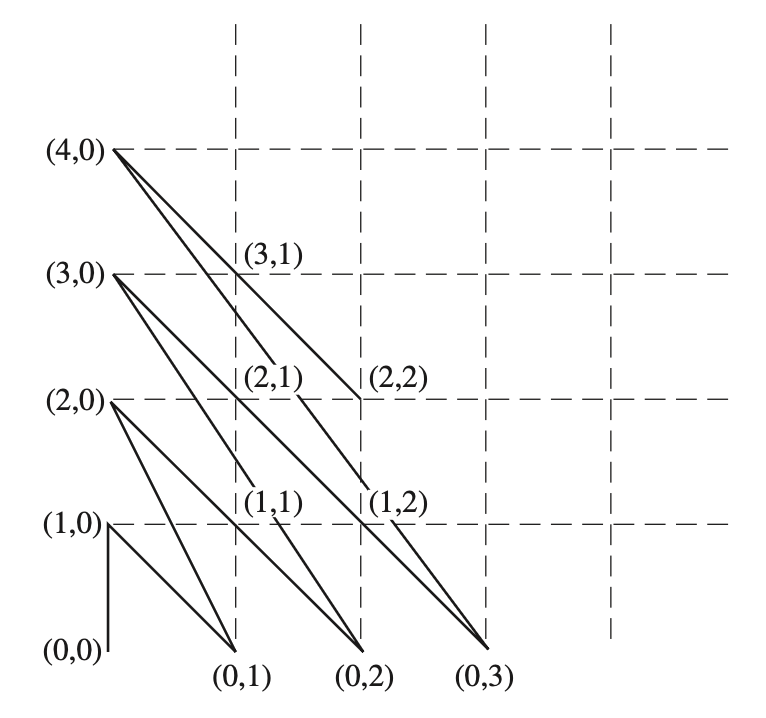
\includegraphics[width=0.4\linewidth]{figures/Figure1.png}
    \caption{Denumerability of $\mathbb N\times\mathbb N$ (pairs are listed along successive diagonals).}
    \label{fig1}
\end{figure}

\begin{remark}
If one of the $X_i$ is countably infinite, then $X$ is also countably infinite by Proposition~1.4(c).
\end{remark}

We now prove the following key theorem.

\begin{theorem}
The set $\mathbb R$ is uncountable.
More precisely, $\operatorname{card}\mathbb R=\operatorname{card}\mathcal P(\mathbb N)$.
\end{theorem}

\begin{proof}
Let $\Phi:\{0,1\}^{\mathbb N}\longrightarrow [0,\tfrac12]$ be defined by
\[
\Phi\bigl((x_n)_{n\ge 0}\bigr)=\sum_{n=0}^{+\infty}\frac{x_n}{3^{n+1}}.
\]
The map $\Phi$ is injective.
Indeed, if $(x_n)_{n\ge 0}\ne (y_n)_{n\ge 0}$ and $\ell:=\min\{\,n\;;\; x_n\ne y_n\,\}$ is finite, then
\[
\bigl|\Phi(x)-\Phi(y)\bigr|
\;\ge\;
\frac{1}{3^{\ell+1}}-\sum_{n=\ell+1}^{+\infty}\frac{1}{3^{n+1}}
\;=\;
\frac{1}{2\cdot3^{\ell+1}}
\;>\;0.
\]
Therefore $\mathcal P(\mathbb N)$, which is equipotent to $\{0,1\}^{\mathbb N}$, injects into the interval $[0,\tfrac12]$ via $\Phi$.
Since $[0,\tfrac12]$ in turn injects into $\mathbb R$ via the canonical inclusion, it follows that
\[
\operatorname{card}\mathbb N < \operatorname{card}\mathcal P(\mathbb N)\le \operatorname{card}\mathbb R.
\]
At this stage $\mathcal P(\mathbb N)$ being uncountable, it is immediate that the same holds for $\mathbb R$.

To establish the equality $\operatorname{card}\mathbb R=\operatorname{card}\mathcal P(\mathbb N)$, we first use the bijection
\[
\varphi:\mathbb R\longrightarrow\,]0,1[,\qquad
x\longmapsto \frac{e^x}{1+e^x}.
\]
It follows that
\[
\operatorname{card}[0,1]\le \operatorname{card}\mathbb R=\operatorname{card}\,]0,1[\,\le \operatorname{card}[0,1[,
\]
and hence $\operatorname{card}\mathbb R=\operatorname{card}[0,1[$.

Now define $\Psi:[0,1[\ \longrightarrow\ \{0,1\}^{\mathbb N}$ by $\Psi(x):=(x_n)_{n\in\mathbb N}$ where
\[
x_0:=\lfloor 2x\rfloor,\qquad
x_n:=\left\lfloor 2^{\,n+1}\!\left(x-\sum_{k=0}^{n-1}\frac{x_k}{2^{\,k+1}}\right)\right\rfloor,\quad n\ge 1.
\]
(Here $\lfloor\cdot\rfloor$ denotes the integer part.)
Then $\Psi(x)$ is the \emph{proper dyadic expansion} of $x$, and we have the equality
\[
x=\sum_{n=0}^{+\infty}\frac{x_n}{2^{\,n+1}},
\]
which in turn implies the injectivity of $\Psi$.
Therefore
\[
\operatorname{card}\mathbb R=\operatorname{card}[0,1[\ \le\ \operatorname{card}\{0,1\}^{\mathbb N}\ =\ \operatorname{card}\mathcal P(\mathbb N).
\]
We conclude that $\operatorname{card}\mathbb R=\operatorname{card}\mathcal P(\mathbb N)$, which completes the proof.
\end{proof}

\newpage
\section{Some complements of topology}

These few reminders and complements cannot in any way replace a course in general topology or in metric structures.
Only the notions that are absolutely indispensable in measure theory and in integration are covered:
the completed line $\overline{\mathbb{R}}$, the upper and lower limits, separability and countable bases of open sets, and finally the distance-to-a-set functions.
Conversely, basic notions such as the adherence (closure) or interior of a set, compactness—of which abundant use will be made later on—are neither developed nor even redefined here.
In case of doubt or omission, one should turn to a textbook in general topology or, more simply, in metric structures.

\subsection{The completed line}

The completed line, generally denoted by $\overline{\mathbb{R}}$, is an ordered metric space meeting three essential requirements:
\begin{itemize}[leftmargin=1.5em]
\item it is a superset of $\mathbb{R}$ that is as ``small'' as possible in the sense of inclusion;
\item it is compact and totally ordered;
\item it is compatible with the real line in the sense that the order and the topology on $\overline{\mathbb{R}}$, when restricted to $\mathbb{R}$, coincide with the natural order on $\mathbb{R}$ and with the topology associated with the absolute-value metric.
\end{itemize}

There are several ways to proceed which, more or less, all amount to constructing a homeomorphism between $\mathbb{R}$ and some open interval of $\mathbb{R}$ that one then extends suitably.
Consider, for example, the map
\[
f:\ \mathbb{R}\longrightarrow (-1,1),\qquad
x\longmapsto \frac{x}{\sqrt{x^2+1}}\, .
\]

The function $f$ is clearly a homeomorphism between $\mathbb{R}$ and $(-1,1)$ (its inverse
$f^{-1}(y):=\dfrac{y}{\sqrt{1-y^2}}$ is indeed continuous).
Now, since the open interval $(-1,1)$ has $[-1,1]$ as its closure in $\mathbb{R}$, the idea to build $\overline{\mathbb{R}}$ is to add two elements, denoted $-\infty$ and $+\infty$, to $\mathbb{R}$ so as to make them the preimages of $-1$ and $1$ under an extension $\tilde f$ of $f$ to $\overline{\mathbb{R}}$.

We therefore set
\begin{equation}\label{eq:2.1}
\overline{\mathbb{R}}:=\mathbb{R}\cup\{+\infty,-\infty\},
\qquad
\tilde f\big|_{\mathbb{R}}:=f,\qquad
\tilde f(-\infty):=-1,\ \ \tilde f(+\infty):=1 .
\end{equation}

What remains—and this is the most important part—is to define on $\overline{\mathbb{R}}$ a total order, denoted $\le$, and a distance $\delta$.

\medskip\noindent
\textit{Order on $\overline{\mathbb{R}}$.}
\[
\begin{cases}
\text{(i) the usual order on }\mathbb{R},\text{ i.e.\ }x\le y\text{ iff }y-x\in\mathbb{R}_+\ \text{for }x,y\in\mathbb{R},\\[2pt]
\text{(ii) for all }x\in\overline{\mathbb{R}}\setminus\mathbb{R}:\ -\infty\le x\le +\infty .
\end{cases}
\]

\medskip\noindent
\textit{Distance on $\overline{\mathbb{R}}$.}
\begin{equation}\label{eq:2.2}
\forall x,y\in\overline{\mathbb{R}},\qquad
\delta(x,y):=\bigl|\tilde f(x)-\tilde f(y)\bigr|.
\end{equation}

The next proposition shows that the desired goal is achieved.

\begin{proposition}
\begin{itemize}[leftmargin=1.5em]
\item[(a)] The binary relation $\le$ is a total order on $\overline{\mathbb{R}}$, for which every nonempty subset has a least upper bound and a greatest lower bound, and $\delta$ is a distance on $\overline{\mathbb{R}}$.
\item[(b)] The identity map $Id:(\mathbb{R},\,\delta\!\big|_{\mathbb{R}})\to(\mathbb{R},\,|\cdot|)$ is a homeomorphism.
\item[(c)] The space $(\overline{\mathbb{R}},\delta)$ is compact, homeomorphic to the interval $[-1,1]$, and $\mathbb{R}$ is open in $\overline{\mathbb{R}}$.
There exists a homeomorphism compatible with the orders on $\overline{\mathbb{R}}$ and $[-1,1]$; this is the case for the map $\tilde f$ defined by \eqref{eq:2.1}.
\end{itemize}
\end{proposition}

\begin{proof}
\begin{itemize}
\item (a) That $\le$ is a total order is immediate.
Moreover, any nonempty subset of $\overline{\mathbb{R}}$ is either bounded above in $\mathbb{R}$ and thus has a least upper bound in $\mathbb{R}$, or not bounded above in $\mathbb{R}$ and then admits $+\infty$ as an upper bound in $\overline{\mathbb{R}}$; similarly for the greatest lower bound.
As for the distance, it suffices to note that $\tilde f$ is injective from $\overline{\mathbb{R}}$ into $[-1,1]$ because $f$ maps $\mathbb{R}$ into $(-1,1)$.
This ensures that $\delta(x,y)=0$ if and only if $x=y$.

\item (b) In view of the definition of $\delta$ on $\mathbb{R}$, the bi-continuity of the identity between $\delta$ and $|\cdot|$ consists simply in showing that $f$ is a homeomorphism between $\mathbb{R}$ and $(-1,1)$.
This was established at the beginning of the subsection.
The topology induced by $\delta$ on $\overline{\mathbb{R}}$ thus coincides, on $\mathbb{R}$, with the one defined by the absolute value.

\item (c) The map $\tilde f$ is clearly a strictly increasing bijection between $\overline{\mathbb{R}}$ and $[-1,1]$.
Finally, for all $x,y\in\overline{\mathbb{R}}$,
\[
|\tilde f(x)-\tilde f(y)|=\delta(x,y),
\]
so $\tilde f$ is an isometry; hence it is a homeomorphism.
\end{itemize}
\end{proof}

It follows immediately that $\overline{\mathbb{R}}=\tilde f^{-1}([-1,1])$ is a compact interval since the inverse map $\tilde f^{-1}$ is continuous.
Finally, $\mathbb{R}$, being the inverse image of $(-1,1)$ under the continuous map $\tilde f$, is open in $\overline{\mathbb{R}}$.

From point (b) we immediately obtain the following corollary, where $\mathcal{O}_\delta(X)$ denotes the family of open sets of the topology on $X$ defined by the distance $d$ (see \S\,\ref{sec:2.3} just below).

\begin{corollary}
\[
\mathcal{O}_\delta(\overline{\mathbb{R}})\cap \mathbb{R}=\mathcal{O}_{|\cdot|}(\mathbb{R}).
\]
\end{corollary}

\begin{proof}
Indeed, if $i:\mathbb{R}\hookrightarrow \overline{\mathbb{R}}$ denotes the canonical injection, then for every $O\in\mathcal{O}(\overline{\mathbb{R}})$ one has $i^{-1}(O)=O\cap\mathbb{R}\in\mathcal{O}(\mathbb{R})$.
Conversely, since $\mathbb{R}$ is open in $\overline{\mathbb{R}}$, every open set $O$ of $\mathbb{R}$ is open in $\overline{\mathbb{R}}$; it is therefore the trace on $\mathbb{R}$ of itself.
\end{proof}

\subsection{Upper and lower limits}

From now on, $\overline{\mathbb{R}}$ is endowed with the distance $\delta$ defined by \eqref{eq:2.2}, which is compatible with the order on $\overline{\mathbb{R}}$ and makes it a compact metric space.

\begin{definition}
Let $(x_n)_{n\in\mathbb{N}}$ be a sequence of elements of $\overline{\mathbb{R}}$.
We define the \emph{upper limit} of the sequence $(x_n)_{n\in\mathbb{N}}$ by
\[
\limsup_{n\to\infty} x_n:=\inf_{n\ge 0}\Bigl(\sup_{k\ge n} x_k\Bigr)\in\overline{\mathbb{R}},
\]
and the \emph{lower limit} of the sequence $(x_n)_{n\in\mathbb{N}}$ by
\[
\liminf_{n\to\infty} x_n:=\sup_{n\ge 0}\Bigl(\inf_{k\ge n} x_k\Bigr)\in\overline{\mathbb{R}}.
\]
\end{definition}

\begin{remark}
Since every monotone sequence of $\overline{\mathbb{R}}$ converges, we immediately have
\[
\limsup_{n\to\infty} x_n=\lim_{n\to\infty}^{\downarrow}\Bigl(\sup_{k\ge n} x_k\Bigr)
\qquad\text{and}\qquad
\liminf_{n\to\infty} x_n=\lim_{n\to\infty}^{\uparrow}\Bigl(\inf_{k\ge n} x_k\Bigr).
\]
\end{remark}

The following result links upper and lower limits with monotonicity and continuity; it will be useful later.

\begin{proposition}
Let $(x_n)_{n\in\mathbb{N}}$ be a sequence of elements of $\overline{\mathbb{R}}$, and let $f:\overline{\mathbb{R}}\to\overline{\mathbb{R}}$ be a monotone and continuous function.
Then
\[
\begin{aligned}
&f\!\left(\limsup_{n} x_n\right)=\limsup_{n} f(x_n)
\quad\text{and}\quad
f\!\left(\liminf_{n} x_n\right)=\liminf_{n} f(x_n)
&&\text{if $f$ is increasing,}\\
&f\!\left(\limsup_{n} x_n\right)=\liminf_{n} f(x_n)
\quad\text{and}\quad
f\!\left(\liminf_{n} x_n\right)=\limsup_{n} f(x_n)
&&\text{if $f$ is decreasing.}
\end{aligned}
\]
\end{proposition}

\begin{proof}
We treat the case of the upper limit when $f$ is increasing; the other cases are similar.
Set $y_n:=\sup_{k\ge n} x_k$, $n\in\mathbb{N}$.
The monotonicity of $f$ implies $f(y_n)\ge \sup_{k\ge n} f(x_k)$.
Moreover, by the definition of the least upper bound, there exists a subsequence $(x_{\varphi(k)})$ extracted from $(x_k)_{k\ge n}$ that converges to $y_n$ in $\overline{\mathbb{R}}$ (with $n$ fixed).
Hence $f(y_n)=\lim_{k} f(x_{\varphi(k)})\le \sup_{k\ge n} f(x_k)$ by continuity of $f$.
Thus $f(y_n)=\sup_{k\ge n} f(x_k)$.
Again by the continuity of $f$ we have
\[
\lim_{n} f(x_n)=\lim_{n}^{\downarrow}\sup_{k\ge n} f(x_k)=\lim_{n}^{\downarrow} f(y_n)=f\!\left(\lim_{n}^{\downarrow} y_n\right)=f\!\left(\limsup_{n} x_n\right),
\]
which yields the desired equality.
\end{proof}

The interest of upper and lower limits lies essentially in the following result.

\begin{proposition}
Let $(x_n)_{n\in\mathbb{N}}$ be a sequence of elements of $\overline{\mathbb{R}}$.
Then $\limsup_{n} x_n$ and $\liminf_{n} x_n$ are respectively the largest and the smallest cluster values of the sequence $(x_n)_{n\in\mathbb{N}}$ in $\overline{\mathbb{R}}$.
Moreover,
\[
(x_n)_{n\in\mathbb{N}}\ \text{converges in }\overline{\mathbb{R}}
\quad\Longleftrightarrow\quad
\limsup_{n} x_n=\liminf_{n} x_n .
\]
\end{proposition}

\begin{proof}
Since $(\overline{\mathbb{R}},\delta)$ is compact, the sequence $(x_n)$ has a cluster value (Bolzano--Weierstrass theorem).
Let $\ell$ be a cluster value of $(x_n)$.
There exists an extracted subsequence $(x_{\varphi(n)})$ which converges to $\ell$ in $(\overline{\mathbb{R}},\delta)$.
Given that $x_{\varphi(n)}\le \sup_{k\ge \varphi(n)} x_k$, which decreases to $\limsup_{n} x_n$, we obtain, using the compatibility of the topology on $\overline{\mathbb{R}}$ with the order on $\overline{\mathbb{R}}$, that
\[
\ell \le \limsup_{n} x_n.
\]
We now show that $\ell_+:=\limsup_{n} x_n$ is itself a cluster value of $(x_n)$.
By the characterization of a cluster value in a metric space, this means:
\[
\forall \varepsilon>0,\ \forall N\in\mathbb{N},\ \exists n\ge N\ \text{such that}\ \delta(x_n,\ell_+)\le \varepsilon.
\]
Set $y_n:=\tilde f(x_n)\in[-1,1]$, $n\in\mathbb{N}$, where $\tilde f$ is defined in \eqref{eq:2.1}.
By Proposition~\ref{eq:2.2} (i.e.\ by \eqref{eq:2.2}) and Proposition~2.2, we have $\lim_{n}^\downarrow y_n=\tilde f(\ell_+)$ because $\tilde f$ is increasing and continuous on $\overline{\mathbb{R}}$.
Consequently, the sequence with general term $z_n:=\sup_{k\ge n} y_k$ decreases to $\tilde f(\ell_+)$.
Let $\varepsilon>0$ and $N\in\mathbb{N}$.
There exists $n_0\ge N$ such that, for all $n\ge n_0$, $\tilde f(\ell_+)\le z_n\le \tilde f(\ell_+)+\varepsilon$.
Moreover, by the definition of the supremum, there exists $n\ge n_0$ such that $y_n\le z_n\le y_n+\varepsilon$.
Hence we can choose $n\ge N$ so that
\[
\tilde f(\ell_+) - \varepsilon \le z_n - \varepsilon \le y_n \le z_n \le \tilde f(\ell_+)+\varepsilon,
\]
which implies $\delta(x_n,\ell_+)=|y_n-\tilde f(\ell_+)|\le \varepsilon$.
An equivalent result holds for the lower limit upon noting that
\[
\liminf_{n} x_n= -\,\limsup_{n}(-x_n).
\]
Finally, since $(\overline{\mathbb{R}},\delta)$ is compact, the sequence $(x_n)$ converges if and only if it admits a unique cluster value; that is, iff $\limsup_{n} x_n=\liminf_{n} x_n$.
\end{proof}

We end this subsection with two properties of upper and lower limits, relative to the operations $+$ and $\times$.

\begin{proposition}
\begin{itemize}[leftmargin=1.5em]
\item[(a)] Let $(x_n)_{n\in\mathbb{N}}$ and $(y_n)_{n\in\mathbb{N}}$ be two sequences in $\overline{\mathbb{R}}$ which are simultaneously bounded above in $[-\infty,+\infty[$ (or simultaneously bounded below in $]-\infty,+\infty]$).
Then
\[
\limsup_{n}(x_n+y_n)\ \le\ \limsup_{n} x_n + \limsup_{n} y_n,
\qquad
\liminf_{n}(x_n+y_n)\ \ge\ \liminf_{n} x_n + \liminf_{n} y_n .
\]
\item[(b)] Let $(x_n)_{n\in\mathbb{N}}$ and $(y_n)_{n\in\mathbb{N}}$ be two sequences in $\mathbb{R}_+$, simultaneously bounded above in $\mathbb{R}_+$ (or simultaneously bounded below in $]0,+\infty]$).
Then
\[
\limsup_{n}(x_n y_n)\ \le\ \bigl(\limsup_{n} x_n\bigr)\bigl(\limsup_{n} y_n\bigr),
\qquad
\liminf_{n}(x_n y_n)\ \ge\ \bigl(\liminf_{n} x_n\bigr)\bigl(\liminf_{n} y_n\bigr).
\]
\end{itemize}
\end{proposition}

\begin{proof}
\begin{itemize}
\item (a) follows from the estimates
\[
\sup_{k\ge n}(x_k+y_k)\ \le\ \sup_{k\ge n} x_k + \sup_{k\ge n} y_k,
\qquad
\inf_{k\ge n}(x_k+y_k)\ \ge\ \inf_{k\ge n} x_k + \inf_{k\ge n} y_k.
\]

\item (b) is obtained by applying (a) to the sequences $\ln(x_n)$ and $\ln(y_n)$—with the conventions $\ln(0)=-\infty$ and $\ln(+\infty)=+\infty$—and then applying Proposition~2.2 successively to the functions $\ln$ and $\exp$.
\end{itemize}
\end{proof}

\subsection{Topology on a set. Metric space}\label{sec:2.3}

\begin{definition}
\begin{itemize}[leftmargin=1.5em]
\item[(a)] A \emph{topology} on a set $X$ is a family $\mathcal{O}(X)$ of subsets of $X$ satisfying
\begin{itemize}[leftmargin=1.2em]
\item[(i)] $\varnothing$ and $X$ belong to $\mathcal{O}(X)$;
\item[(ii)] for every $n\in\mathbb{N}^{\!*}$, if $O_1,\dots,O_n\in\mathcal{O}(X)$ then $\displaystyle \bigcap_{i=1}^n O_i\in\mathcal{O}(X)$ \quad[stability under finite intersections];
\item[(iii)] for any index set $I$, if $O_i\in\mathcal{O}(X)$ for every $i\in I$, then $\displaystyle \bigcup_{i\in I} O_i\in\mathcal{O}(X)$ \quad[stability under arbitrary unions].
\end{itemize}
\item[(b)] The elements of $\mathcal{O}(X)$ are called the \emph{open sets} of $X$.
The complements of open sets are called \emph{closed} sets.
\item[(c)] A topology is \emph{separated} (Hausdorff) if two distinct points of $X$ belong to two disjoint open sets.
\end{itemize}
\end{definition}

\begin{example}[from the metric case]
If $(X,d)$ is a metric space,\footnote{Recall that a distance is a map $d:X\times X\to\mathbb{R}_+$ such that:
$d(x,y)=0$ iff $x=y$; $d(x,y)=d(y,x)$; $d(x,y)\le d(x,z)+d(z,y)$ for all $x,y,z\in X$.}
the topology on $X$ associated with $d$ is given by the family of open sets
\[
\mathcal{O}_d(X):=\left\{\ \bigcup_{i\in I} \mathring{B}(x_i,r_i)\,,\ x_i\in X,\ r_i\in\mathbb{R}_+^{\!*},\ I\text{ arbitrary}\right\},
\]
where $\mathring{B}(x,r)=\{\,y\in X: d(x,y)<r\,\}$.
One checks that this family satisfies the axioms of a separated topology.
Moreover, it is clear that, in this framework,
\[
O\in\mathcal{O}_d(X)\quad\Longleftrightarrow\quad
\forall x\in O,\ \exists r_x>0\ \text{such that}\ \mathring{B}(x,r_x)\subset O .
\]

\end{example}

\subsection{Countable base of open sets; separability}

\begin{definition}
\begin{itemize}[leftmargin=1.5em]
\item[(a)] A topological space $(X,\mathcal{O}(X))$ is said to have a \emph{countable base of open sets} if there exists a countable family of nonempty open sets $\{\omega_n,\ n\ge 1\}$ such that
\[
\forall O\in\mathcal{O}(X),\ \exists I\subset\mathbb{N}\ \text{with}\ O=\bigcup_{n\in I}\omega_n .
\]
\item[(b)] A metric space $(X,d)$ is \emph{separable} if it contains a dense sequence $(x_n)_{n\in\mathbb{N}}$.\footnote{Recall that a sequence $(x_n)$ is dense in $X$ if, for every $x\in X$, there exists an extracted subsequence $(x_{\varphi(n)})$ such that $d(x_{\varphi(n)},x)\to 0$.}
\end{itemize}
\end{definition}

\begin{proposition}
A metric space is separable if and only if it has a countable base of open sets.
\end{proposition}

\begin{proof}
($\Rightarrow$) One verifies that a countable base of open sets is made of the balls
$\{\mathring{B}(x_n,r):\ n\in\mathbb{N},\ r\in\mathbb{Q}_+^{\!*}\}$, where $(x_n)$ is a dense sequence.
Indeed, for every open set $O\subset X$,
\[
O=\bigcup_{\mathring{B}(x_n,r)\subset O}\mathring{B}(x_n,r).
\]
As for the countability of $\mathbb{N}\times\mathbb{Q}_+^{\!*}$, it follows from the results on cardinals established in Chapter~2.

($\Leftarrow$) Let $(\omega_n)_{n\in\mathbb{N}}$ be a countable base of open sets.
It is immediate that any sequence $(x_n)$ with $x_n\in\omega_n$ is dense.\end{proof}

\subsection{Examples of topology constructions}

\subsubsection{Induced topology}

\begin{definition}
Let $(X,\mathcal{O}(X))$ be a topological space and let $Y\subset X$ be a subset of $X$.
The \emph{induced topology} (by that of $X$) on $Y$ is defined by
\[
\mathcal{O}(Y):=\{\,O\cap Y\,;\ O\in\mathcal{O}(X)\,\}.
\]
\end{definition}

Note that if $i:Y\hookrightarrow X$ denotes the canonical injection, then
\[
\mathcal{O}(Y)=\{\,i^{-1}(O),\ O\in\mathcal{O}(X)\,\}=i^{-1}\bigl(\mathcal{O}(X)\bigr).
\]
Moreover, a topology induced by a separated topology is itself separated.

\medskip\noindent
\textit{Metric case.}
If the topology on $X$ is the metric topology relative to a distance $d$, one checks immediately that
$\mathcal{O}(Y)=\mathcal{O}_{\,d|_Y}(Y)$, where $d|_Y$ denotes the restriction to $Y$ of the distance $d$.

\medskip\noindent
\textit{Induced topology and separability.}
If $(X,d)$ is separable, it has a countable base of open sets.
By the very definition of the induced topology, if $(\omega_n)_{n\in\mathbb{N}}$ is a countable base of open sets of $X$, then $(\omega_n\cap Y)_{n\in\mathbb{N}}$ is a countable base of open sets of $Y$, hence $(Y,d)$ is separable.

\subsubsection{Product topology}

\begin{definition}
If $(X,\mathcal{O}(X))$ and $(Y,\mathcal{O}(Y))$ are two topological spaces, the \emph{product topology} on $X\times Y$ is defined by the family of open sets
\[
\mathcal{O}(X\times Y):=\left\{\ \bigcup_{i\in I}\bigl(O_i\times \Omega_i\bigr),\ O_i\in\mathcal{O}(X),\ \Omega_i\in\mathcal{O}(Y),\ I\ \text{arbitrary}\ \right\}.
\]
\end{definition}

\noindent\textbf{Remarks.}
\begin{itemize}[leftmargin=1.5em]
\item The product topology arising from two separated topologies is itself separated.
\item The product topology on $X\times Y$ is the smallest topology on $X\times Y$ that makes the canonical projections $\pi_X$ and $\pi_Y$ continuous from $X\times Y$ to the topological spaces $(X,\mathcal{O}(X))$ and $(Y,\mathcal{O}(Y))$ respectively.
\end{itemize}

If the topologies on $X$ and $Y$ are metric relative to distances $d$ and $\delta$, one verifies immediately that $\mathcal{O}(X\times Y)$ is also the topology associated with the usual distances on $X\times Y$, such as
\[
\begin{aligned}
D_1\bigl((x,y),(x',y')\bigr)&:= d(x,x')+\delta(y,y'),\\
D_p\bigl((x,y),(x',y')\bigr)&:= \bigl((d(x,x')^p+\delta(y,y')^p\bigr)^{1/p},\quad p\in[1,+\infty[,\\
D_\infty\bigl((x,y),(x',y')\bigr)&:= \max\{\,d(x,x'),\,\delta(y,y')\,\},
\end{aligned}
\]
and many other distances on $X\times Y$ define this same product topology.

\begin{proposition}
\begin{itemize}[leftmargin=1.5em]
\item[(a)] If $(X,\mathcal{O}(X))$ and $(Y,\mathcal{O}(Y))$ each have a countable base of open sets, then $(X\times Y,\mathcal{O}(X\times Y))$ has a countable base of open sets.
\item[(b)] If $(X,d)$ and $(Y,\delta)$ are separable, then $X\times Y$ is separable for all (topologically) equivalent distances defining the product topology, e.g.\ the $D_p$, $p\in[1,+\infty[$.
\end{itemize}
\end{proposition}

\begin{proof}
\begin{itemize}
\item (a) Let $\mathcal{U}_X:=\{U_n, n\ge 1\}$ and $\mathcal{U}_Y:=\{V_n, n\ge 1\}$ be countable bases of open sets for $X$ and $Y$, respectively.
Then the countable family $\mathcal{U}_X\times\mathcal{U}_Y:=\{U_n\times V_m,\ (n,m)\in\mathbb{N}^2\}$ is a base of open sets for $\mathcal{O}(X\times Y)$.
Indeed, if $O\in\mathcal{O}(X\times Y)$ and $z=(x,y)\in O=\bigcup_{i\in I} O_i\times\Omega_i$, there exists $i_z\in I$ such that $(x,y)\in O_{i_z}\times\Omega_{i_z}$; by definition of the bases $\mathcal{U}_X$ and $\mathcal{U}_Y$, there exist integers $n_x$ and $m_y$ such that $x\in U_{n_x}\subset O_{i_z}$ and $y\in V_{m_y}\subset \Omega_{i_z}$.
Finally,
\[
O=\bigcup_{(x,y)\in O} U_{n_x}\times V_{m_y}=\bigcup_{(n,m)\in\mathcal{L}_O} U_n\times V_m,
\]
where $\mathcal{L}_O:=\{(n_x,m_y),\ (x,y)\in O\}\subset\mathbb{N}^2$.

\item (b) This point is an immediate corollary of (a) and Proposition~2.5.
One can also proceed directly: if $\{x_n, n\ge 1\}$ and $\{y_n, n\ge 1\}$ are dense sequences in $(X,d)$ and $(Y,\delta)$, then by the very definition of the distances $D_p$, the set $\{(x_n,y_m),\ n,m\ge 1\}$ is dense in $(X\times Y, D_p)$.
\end{itemize}
\end{proof}

\subsection{Distance from a point to a set}

\begin{definition}
Let $(X,d)$ be a metric space and let $A$ be a nonempty subset of $X$.
For every $x\in X$ we define the distance from $x$ to $A$ by
\[
d(x,A):=\inf_{a\in A} d(x,a)\ \in [0,+\infty[\, .
\]
\end{definition}

These functions arise very often in measure theory, for they provide an efficient way to approximate indicator functions of sets by continuous functions.

\begin{proposition}
\begin{itemize}[leftmargin=1.5em]
\item[(a)] For every nonempty subset $A$ of $X$, the map $x\mapsto d(x,A)$, with values in $\mathbb{R}_+$, is $1$-Lipschitz with respect to the distance $d$, i.e.
\[
\forall x,y\in X,\qquad |\,d(x,A)-d(y,A)\,|\le d(x,y).
\]
\item[(b)] The set $\{x\in X:\ d(x,A)=0\}$ is equal to $\overline{A}$ (the closure of $A$ in $X$).
\end{itemize}
\end{proposition}

\begin{proof}
\begin{itemize}
\item (a) For any $z\in A$, $d(x,A)\le d(x,z)\le d(x,y)+d(y,z)$.
Hence $d(x,A)-d(y,A)$ is a lower bound of $\{d(y,z),\ z\in A\}$.
Therefore $d(x,A)-d(y,A)\le d(y,A)$, and finally $d(x,A)-d(y,A)\le d(x,y)$.
Since the roles of $x$ and $y$ are symmetric, the inequality holds in absolute value.

\item (b) Since $d(x,A)$ is always nonnegative, it follows from the definition of the infimum that $d(x,A)=0$ if and only if there exists a sequence $(a_n)_{n\in\mathbb{N}}$ in $A$ such that $\lim_{n} d(x,a_n)=0$.
The result follows, by the definition of the adherence (closure) of $A$ in a metric space.
\end{itemize}
\end{proof}

Other properties of these functions will be established as needed, but all of them rely on Proposition~2.7.

\newpage
\section{Sigma-algebras of subsets of a set}
\subsection{Set-theoretic preliminaries}
In this preliminary paragraph we collect the results concerning the handling of sets and functions that prove absolutely indispensable for measure theory and integration. They are essentially reminders.

\medskip\noindent
\begin{itemize}
\item (a) Let $X$ be a set, $\mathcal P(X)$ its power set, and let $A,B\in\mathcal P(X)$. We write
\[
\begin{aligned}
A\cup B &:= \{x\in X: x\in A\ \text{or}\ x\in B\},\\
A\cap B &:= \{x\in X: x\in A\ \text{and}\ x\in B\},\\
{}^{c}\!A &:= \{x\in X: x\notin A\},\\
A\setminus B &:= \{x\in X: x\in A\ \text{and}\ x\notin B\}=A\cap{}^{c}\!B,\\
A\triangle B &:= \{x\in X: x\in A\cup B\ \text{and}\ x\notin A\cap B\}\\
&\phantom{:}= (A\cup B)\setminus(A\cap B)=(A\setminus B)\cup(B\setminus A).
\end{aligned}
\]
\medskip\noindent
\item (b) Let $f:X\to Y$, $A_i\subset X$, $B_i\subset Y$, $i\in I$ ($I$ any index set). With $f$ we canonically associate the set-maps “direct image’’ $f_d$ and “inverse image’’ $f_r^{-1}$ defined by
\[
\begin{aligned}
f_d:\ \mathcal P(X) &\longrightarrow \mathcal P(Y), & A &\longmapsto f_d(A):=\{f(x):x\in A\},\\
f_r^{-1}:\ \mathcal P(Y) &\longrightarrow \mathcal P(X), & B &\longmapsto f_r^{-1}(B):=\{x\in X: f(x)\in B\}.
\end{aligned}
\]
(For simplicity, and despite the risk of confusion, we almost always write $f$ instead of $f_d$ and $f^{-1}$ instead of $f_r^{-1}$.)

These set-maps $f_d$ and $f_r^{-1}$ satisfy Hausdorff’s formulas: if $(A_i)_{i\in I}$ is a family of subsets of $X$ and $(B_j)_{j\in J}$ a family of subsets of $Y$ ($I$ and $J$ assumed nonempty), then
\[
\left\{
\begin{aligned}
&f_d\!\Bigl(\bigcup_{i\in I}A_i\Bigr)=\bigcup_{i\in I} f_d(Ai),\qquad
&&f_d\!\Bigl(\bigcap_{i\in I}A_i\Bigr)\subset\bigcap_{i\in I} f_d(A_i)\ \ \text{(with equality if $f$ is injective)},\\
&f_r^{-1}\!\Bigl(\bigcup_{j\in J}B_j\Bigr)=\bigcup_{j\in J} f_r^{-1}(B_j),\qquad
&&f_r^{-1}\!\Bigl(\bigcap_{j\in J}B_j\Bigr)=\bigcap_{j\in J} f_r^{-1}(B_j),\\
&{}^{c}\!f_r^{-1}(B)=f_r^{-1}({}^{c}\!B).
\end{aligned}
\right.
\]
Finally, when $f$ is bijective there is a simple link between the set-map $f_r^{-1}$ and the reciprocal $f^{-1}$ of $f$: for every subset $B$ of $Y$,
\[
f_r^{-1}(B)=\{\,f^{-1}(b): b\in B\,\}.
\]

\begin{notation}
	If $\mathscr C\subset\mathcal P(Y)$ is a family of subsets of $Y$, we extend the notation by
\[
f^{-1}(\mathscr C):=\{\,f^{-1}(C): C\in\mathscr C\,\}\subset\mathcal P(X).
\]

\medskip\noindent
\item (c) Let $(A_n)_{n\ge1}$ be a (countable) sequence of subsets. We define the “upper’’ and “lower’’ limits of $A_n$ by
\[
\begin{aligned}
\limsup_{n} A_n
&:= \bigcap_{n\ge1}\ \bigcup_{k\ge n} A_k
= \{\,x\in X: \forall n\ge1,\ \exists k\ge n\ \text{with } x\in A_k\,\}\\
&= \{\,x\in X: x\in A_k\ \text{infinitely often}\,\},\\[3pt]
\liminf_{n} A_n
&:= \bigcup_{n\ge1}\ \bigcap_{k\ge n} A_k
= \{\,x\in X: \exists n\ge1,\ \forall k\ge n,\ x\in A_k\,\}\\
&= \{\,x\in X: x\in A_k\ \text{from some rank on}\,\}.
\end{aligned}
\]
One checks immediately that $\liminf_{n} A_n\subset\limsup_{n} A_n$, and one speaks of the limit $\lim_{n} A_n$ in case of equality between $\liminf_{n} A_n$ and $\limsup_{n} A_n$.
Moreover, if $(A_n)_{n\ge1}$ is increasing (resp.\ decreasing) for inclusion, then
\[
\lim_{n} A_n=\liminf_{n} A_n=\bigcup_{n\ge1} A_n
\quad\text{(resp.\ } \lim_{n} A_n=\limsup_{n} A_n=\bigcap_{n\ge1} A_n\text{)}.
\]

\medskip\noindent
\item (d) \textit{De Morgan’s laws:}\quad ${}^{c}\!\bigl(\bigcap_{i\in I}A_i\bigr)=\bigcup_{i\in I}{}^{c}\!A_i$ and ${}^{c}\!\bigl(\bigcup_{i\in I}A_i\bigr)=\bigcap_{i\in I}{}^{c}\!A_i$.
Hence
\[
{}^{c}\!\bigl(\limsup\nolimits_{n}A_n\bigr)=\liminf\nolimits_{n}{}^{c}\!A_n,
\qquad
{}^{c}\!\bigl(\liminf\nolimits_{n}A_n\bigr)=\limsup\nolimits_{n}{}^{c}\!A_n.
\]
\end{itemize}
\end{notation} 

\subsection{Sigma-algebra and Borel sigma-algebra}\label{subsec:3.1}

\begin{definition}
\begin{itemize}
\item (a) Let $X$ be a set. A \emph{sigma-algebra} (or \emph{$\sigma$-algebra}) on $X$ is any family $\mathcal A$ of subsets of $X$ satisfying:
\begin{itemize}[leftmargin=1.5em]
\item[(i)] $\varnothing\in\mathcal A$;
\item[(ii)] if $A\in\mathcal A$ then ${}^{c}\!A\in\mathcal A$ \hfill[stability under complement];
\item[(iii)] if $(A_n)_{n\ge1}\in\mathcal A^{\mathbb N^{\!*}}$ then $\displaystyle \bigcup_{n\ge1} A_n\in\mathcal A$ \hfill[stability under countable union].
\end{itemize}
\item (b) The pair $(X,\mathcal A)$ is called a \emph{measurable space} (in the sense “susceptible of receiving a measure’’).
\end{itemize}
\end{definition}

\begin{remark} 
Condition (iii) entails stability of $\mathcal A$ under finite unions. Indeed, fixing $n_0$, set $A_n=\varnothing$ for $n>n_0$.
\end{remark}

\begin{example}[sigma-algebras]

\begin{enumerate}[leftmargin=1.5em,label=\arabic*.]
\item $\mathcal A:=\{\varnothing,X\}$, the coarse sigma-algebra.
\item $\mathcal A:=\mathcal P(X)$, the trivial sigma-algebra.
\item For fixed $A\subset X$, $\mathcal A:=\{\varnothing,X,A,{}^{c}\!A\}$: the smallest sigma-algebra containing the subset $A$.
\item If $X=\bigcup_{i\in I} X_i$, with $I$ nonempty, finite or countably infinite, and $X_i\cap X_j=\varnothing$ for $i\ne j$ (so the $X_i$ form a partition of $X$), then
\[
\mathcal A:=\Bigl\{\ \bigcup_{j\in J} X_j,\ J\subset I\ \Bigr\}
\]
is a sigma-algebra.
\item $\mathcal A:=\{A\in\mathcal P(X): A\ \text{countable or}\ {}^{c}\!A\ \text{countable}\}$.
The only axiom to verify is (iii). Let $(A_n)_{n\ge1}$ be a sequence in $\mathcal A$.
If all $A_n$ are countable, then so is their union (see Proposition~3.5 of Chapter~2).
If one of the $A_n$, say $A_{n_0}$, is not countable, then its complement is.
Consequently ${}^{c}\!\bigl(\bigcup_n A_n\bigr)=\bigcap_n {}^{c}\!A_n\subset {}^{c}\!A_{n_0}$ is necessarily countable.
Moreover, one can show that $\mathcal A\ne\mathcal P(X)$ if and only if $X$ has a non-denumerable infinite cardinal (a noticeably less trivial result beyond the scope of this book).
\item If $(\mathcal A_i)_{i\in I}$ is any family of sigma-algebras on $X$, $I\ne\varnothing$, then $\displaystyle \mathcal A:=\bigcap_{i\in I}\mathcal A_i$ is a sigma-algebra.
\end{enumerate}
\end{example}

\begin{properties}
Let $\mathcal A$ be a sigma-algebra on $X$.
\begin{enumerate}[label=(\alph*),leftmargin=2em]
\item $X\in\mathcal A$.
\item If $A_n\in\mathcal A$ for every $n\in\mathbb N$, then $\displaystyle \bigcap_{n\in\mathbb N} A_n\in\mathcal A$ \hfill[stability under countable intersections by taking $A_n:=X$ for $n>n_0$].
\item If $A,B\in\mathcal A$, then $A\setminus B=A\cap{}^{c}\!B\in\mathcal A$.
\item If $A,B\in\mathcal A$, then $A\triangle B:=(A\setminus B)\cup(B\setminus A)\in\mathcal A$.
\item If $A_n\in\mathcal A$ for all $n$, then $\limsup_{n} A_n\in\mathcal A$ and $\liminf_{n} A_n\in\mathcal A$.
\end{enumerate}
	
\end{properties}

\begin{proof}
\begin{itemize}
\item (a) $X={}^c\!\varnothing\in\mathcal A$. \quad
\item (b) ${}^{c}\!\bigl(\bigcap_{n\in\mathbb N}A_n\bigr)=\bigcup_{n\in\mathbb N} {}^{c}\!A_n\in\mathcal A$.
The points (c), (d), and (e) are immediate.
\end{itemize}
\end{proof}

\medskip\noindent
\begin{remark} [Counterexample]
If $X$ is a topological space\footnote{See Section 2.3.} (or simply metric), the family $\mathcal O(X):=\{O\subset\mathcal P(X): O \text{ open in }X\}$ is in general not a sigma-algebra because axiom (ii) fails: if $O$ is open, then ${}^{c}\!O$ is in general not open. For instance, $\mathbb R^\ast\in\mathcal O(\mathbb R)$ but ${}^{c}\!\mathbb R^\ast=\mathbb R_+\notin\mathcal O(\mathbb R)$.
\end{remark}

\begin{proposition}\label{prop:gen}
\textbf{Definition.}\quad
\begin{itemize}
\item (a) Let $\mathscr C\subset\mathcal P(X)$ be a family of subsets of $X$. There exists a smallest sigma-algebra (with respect to inclusion) containing $\mathscr C$. We denote it $\sigma(\mathscr C)$: the sigma-algebra generated by $\mathscr C$.

\item (b) If $\mathcal T$ is a sigma-algebra, then $\sigma(\mathcal T)=\mathcal T$.

\item (c) If $\mathscr C\subset\mathscr F$, then $\sigma(\mathscr C)\subset \sigma(\mathscr F)$. In particular, if $\mathscr C\subset \mathcal T$ and $\mathcal T$ is a sigma-algebra, then $\sigma(\mathscr C)\subset\mathcal T$.
\end{itemize}
\end{proposition}

\noindent\textit{Proof.}
\begin{itemize}
\item (a) Consider
\[
\sigma(\mathscr C):=\bigcap_{\mathcal T\ \text{sigma-algebra},\ \mathscr C\subset\mathcal T}\ \mathcal T .
\]
Since $\mathcal P(X)$ is a sigma-algebra containing $\mathscr C$, the index set is nonempty; by Examples above, $\sigma(\mathscr C)$ is indeed a sigma-algebra and is obviously the smallest one.
The points (b) and (c) follow immediately from the definition of a generated sigma-algebra.

\begin{example}
1. If $A\subset\mathcal P(X)$, $A\ne X$, $A\ne\varnothing$ fixed, the sigma-algebra generated by $\mathscr C:=\{A\}$ is $\mathcal A=\{\varnothing,X,A,{}^{c}\!A\}$.

2. The sigma-algebra generated by the singletons, i.e.\ $\mathscr C:=\{\{x\}:x\in X\}$, is precisely
\[
\mathcal A:=\{A\in\mathcal P(X): A\ \text{countable or}\ {}^{c}\!A\ \text{countable}\}.
\]

\end{example}

\begin{definition}
Let $(X,\mathcal O(X))$ be a topological space. The \emph{Borel sigma-algebra} of $X$, also called the sigma-algebra of Borel sets of $X$, is
\[
\mathcal B(X):=\sigma\bigl(\mathcal O(X)\bigr).
\]
\end{itemize}
\end{definition}

\begin{remark}
\begin{itemize}[leftmargin=1.5em]
\item It is immediate that $\mathcal B(X)=\sigma(\{F\in\mathcal P(X): F\ \text{closed}\})$.
\item In general $\mathcal B(X)\ne\mathcal P(X)$; notably when $X=\mathbb R$. This delicate result can be proved by cardinality arguments: indeed $\mathcal B(\mathbb R)$ and $\mathbb R$ are equipotent, hence
\[
\operatorname{card}\mathcal B(\mathbb R)=\operatorname{card}\mathbb R<\operatorname{card}\mathcal P(\mathbb R)
\]
(see Proposition 2.1).
\end{itemize}

\end{remark}
One can also proceed directly by exhibiting, with the aid of the axiom of choice, a non-Borel set in the future.

\medskip\noindent
\textit{Borel sets of a topological space with a countable base of opens.}
A topological space (or simply metric) $(X,\mathcal O(X))$ is said to have a countable base of open sets if there exists a family $(\omega_n)_{n\in\mathbb N}$ of opens of $X$ such that
\[
\forall O\in\mathcal O(X),\ \exists I\subset\mathbb N,\quad O=\bigcup_{i\in I}\omega_i .
\]
Thus a metric space $(X,d)$ is separable, i.e.\ contains a dense sequence $(x_n)_{n\in\mathbb N}$,\footnote{In the sense that for every $x\in X$ there exists a subsequence $x_{\varphi(n)}\to x$ as $n\to +\infty$.}
and has a countable base of opens since
\[
\bigl\{\mathring B(x_n,r),\ n\in\mathbb N,\ r\in\mathbb Q^{\ast}_+\bigr\}\quad\text{[since $\mathbb N\times\mathbb Q^{\ast}_+$ is denumerable]}
\]
is such a base (see also Section 2.3 for more details).

From the stability of a sigma-algebra under countable union (axiom (iii)) and from the definition of a Borel sigma-algebra we immediately deduce:

\begin{proposition}
Let $X$ be a topological space possessing a countable base $(\omega_n)_{n\in\mathbb N}$ of open sets. Then $\mathcal B(X)=\sigma\bigl(\{\omega_n,\ n\in\mathbb N\}\bigr)$.
\end{proposition}

\begin{application}
We work on the real line $X=\mathbb R$. Every interval $I\subset\mathbb R$ is Borel in $\mathbb R$ since one can always write it as the union of an open interval and at most two singletons (closed). Conversely, certain families of intervals generate the Borel sigma-algebra. Thus
\[
\mathcal B(\mathbb R)
= \sigma\bigl(\{[a,+\infty[,\, a\in\mathbb Q\}\bigr)
= \sigma\bigl(\{]a,+\infty[,\, a\in\mathbb Q\}\bigr)
= \sigma\bigl(\{]-\infty,a],\, a\in\mathbb Q\}\bigr)
= \sigma\bigl(\{]-\infty,a[,\, a\in\mathbb Q\}\bigr).
\]

\end{application}

\begin{proof}

Since $\mathbb Q$ is dense in $\mathbb R$,
\[
\{] \alpha,\beta[,\, \alpha,\beta\in\mathbb Q,\ \alpha<\beta\}
\]
is a countable base of opens of $\mathbb R$. Hence
\[
\mathcal B(\mathbb R)=\sigma\bigl(\{] \alpha,\beta[,\, \alpha,\beta\in\mathbb Q,\ \alpha<\beta\}\bigr).
\]
But $] \alpha,\beta[ = [\alpha,+\infty[ \cap ]-\infty,\beta[$ and
\[
] \alpha,\beta[=\bigcup_{n\ge1} [\alpha+1/n,+\infty[ \cap ]-\infty,\beta[,
\]
so $\sigma(\{[a,+\infty[, a\in\mathbb Q\})\supset \sigma(\{] \alpha,\beta[, \alpha,\beta\in\mathbb Q,\alpha<\beta\})=\mathcal B(\mathbb R)$. The reverse inclusion is immediate since the sets $[\alpha,+\infty[$ are closed in $\mathbb R$. The other equalities are analogous.

\end{proof}

\subsection{Other examples of sigma-algebras}\label{subsec:3.2}

\subsubsection{Inverse-image sigma-algebra}

\begin{proposition}\label{prop:preimage}
Let $f:X\to Y$ and $\mathcal B$ a sigma-algebra on $Y$. Then
\[
\mathcal A:=\{\,f^{-1}(B): B\in\mathcal B\,\}
\]
is a sigma-algebra on $X$.
\end{proposition}

\begin{proof}
The result follows from the “reciprocal’’ Hausdorff formulas recalled at the beginning of this chapter:
\[
{}^{c}\!\bigl(f^{-1}(B)\bigr)= f^{-1}({}^{c}\!B)\in\mathcal A,
\qquad
\bigcup_{n\in\mathbb N} f^{-1}(B_n)= f^{-1}\!\Bigl(\bigcup_{n\in\mathbb N} B_n\Bigr)\in\mathcal A.
\]

\end{proof}

\begin{definition}
The sigma-algebra $\{\,f^{-1}(B),\, B\in\mathcal B\,\}$ is called the \emph{inverse-image sigma-algebra} (understood “of $\mathcal B$ by $f$’’). We denote it $f^{-1}(\mathcal B)$ or $\sigma(f)$.
\end{definition}

\begin{example}
1. \emph{Trace sigma-algebra.} If $Y\subset X$ and $i:Y\to(X,\mathcal A)$ is the inclusion, then $i^{-1}(\mathcal A)=\{A\cap Y,\ A\in\mathcal A\}$: the trace sigma-algebra of $\mathcal A$ on $Y$. If $Y\in\mathcal A$, then $i^{-1}(\mathcal A)\subset\mathcal A$.

2. \emph{Band sigma-algebra.} Let $\pi:X\times Y\to (X,\mathcal A)$ be the canonical projection onto $X$. The band sigma-algebra is $\pi^{-1}(\mathcal A)=\{A\times Y,\ A\in\mathcal A\}$.
\end{example}

\subsubsection{Image sigma-algebra}

The terminology is misleading: if $f:X\to Y$ is a map and $\mathcal A$ a sigma-algebra on $X$, then $\{f(A),\, A\in\mathcal A\}$ is \emph{not} in general a sigma-algebra on $Y$.

\begin{definition}
Let $f:X\to Y$ and $\mathcal A$ a sigma-algebra on $X$. The \emph{image sigma-algebra} of $\mathcal A$ by $f$ is the sigma-algebra on $Y$ defined by
\[
\mathcal B:=\{\,B\in\mathcal P(Y): f^{-1}(B)\in\mathcal A\,\}.
\]
\end{definition}

The family $\mathcal B$ is clearly a sigma-algebra via the “reciprocal’’ Hausdorff formulas.

\subsection{Transport lemma}\label{subsec:3.3}

The following proposition is known as the \emph{transport lemma}.

\begin{proposition}\label{prop:transport}
Let $f:X\to Y$ and $\mathscr C\subset\mathcal P(Y)$. Then
\[
\sigma\bigl(f^{-1}(\mathscr C)\bigr)=f^{-1}\bigl(\sigma(\mathscr C)\bigr)
\qquad\text{[both are sigma-algebras on $X$].}
\]
\end{proposition}

\begin{proof}
We prove the double inclusion.

\noindent$\subset$:\quad $f^{-1}(\mathscr C)\subset f^{-1}(\sigma(\mathscr C))$ hence $\sigma\bigl(f^{-1}(\mathscr C)\bigr)\subset f^{-1}(\sigma(\mathscr C))$ (both sigma-algebras by Proposition~\ref{prop:preimage})

\noindent$\supset$:\quad Consider $\mathcal B$ the image sigma-algebra of $\sigma\bigl(f^{-1}(\mathscr C)\bigr)$ by $f$, i.e.
\[
\mathcal B:=\{\,B\in\mathcal P(Y): f^{-1}(B)\in \sigma\bigl(f^{-1}(\mathscr C)\bigr)\,\}.
\]
Then $\mathscr C\subset\mathcal B$, hence $\sigma(\mathscr C)\subset\mathcal B$ and so $f^{-1}\bigl(\sigma(\mathscr C)\bigr)\subset f^{-1}(\mathcal B)\subset \sigma\bigl(f^{-1}(\mathscr C)\bigr)$ by the very definition of $\mathcal B$.

\medskip\noindent

\end{proof}

\begin{remark}
The statement is easy to retain; the main difficulty lies in understanding the meaning of the two terms.
\end{remark}

\begin{proposition}\label{prop:traceBorel}
\begin{itemize}
\item (a) If $X$ is a metric space and $Y\subset X$ is equipped with the induced distance, then
\[
\mathcal B(Y)=\{\,A\cap Y,\ A\in\mathcal B(X)\,\}.
\]
\item (b) Moreover, $\mathcal B(Y)\subset\mathcal B(X)$ if and only if $Y\in\mathcal B(X)$. In this case,
\[
\mathcal B(Y)=\{\,A\in\mathcal B(X): A\subset Y\,\}.
\]
\end{itemize}
\end{proposition}

\begin{proof}
\begin{itemize}
\item (a) If $i:Y\hookrightarrow X$ denotes the canonical inclusion, then $\mathcal O(Y):=\{O\cap Y,\ O\in\mathcal O(X)\}=i^{-1}\bigl(\mathcal O(X)\bigr)$, hence
\[
\mathcal B(Y)=\sigma\bigl(i^{-1}(\mathcal O(X))\bigr)=i^{-1}\bigl(\sigma(\mathcal O(X))\bigr)=i^{-1}\bigl(\mathcal B(X)\bigr)=\{A\cap Y,\ A\in\mathcal B(X)\}
\]
by the transport lemma (by Proposition 3.4).
\quad

\item (b) is immediate since a sigma-algebra is stable under finite intersection.
\end{itemize}
\end{proof}

\begin{application}
\begin{itemize}
\item (a) \emph{Borel sets of some usual Borel subsets of $\mathbb R$.}
$\mathcal B(\mathbb R_+)=\{A\in\mathcal B(\mathbb R): A\subset \mathbb R_+\}$ since $\mathbb R_+$ is closed in $\mathbb R$ and hence Borel; likewise $\mathcal B(\mathbb R^\ast)=\{A\in\mathcal B(\mathbb R): 0\notin A\}$, etc.

\item (b) \emph{Borel sets of $\overline{\mathbb R}$.}
If $X=\overline{\mathbb R}$ and $Y=\mathbb R$, we are exactly in the setting of Proposition~\ref{prop:traceBorel} as shown by Corollary 3.1. We deduce
\[
\mathcal B(\overline{\mathbb R})\subset\{\,A,\ A\cup\{+\infty\},\ A\cup\{-\infty\},\ A\cup\{\pm\infty\}: A\in\mathcal B(\mathbb R)\,\}.
\]
Conversely, the sets $\{+\infty\}$, $\{-\infty\}$, $\{\pm\infty\}$ are finite and thus closed in $\overline{\mathbb R}$ and therefore Borel. Also, by Proposition~\ref{prop:traceBorel}, $\mathcal B(\mathbb R)\subset \mathcal B(\overline{\mathbb R})$ since $\mathbb R\in\mathcal O(\overline{\mathbb R})\subset\mathcal B(\overline{\mathbb R})$. We obtain a first characterization:
\begin{equation}\label{eq:3.1}
\mathcal B(\overline{\mathbb R})=\{\,A,\ A\cup\{+\infty\},\ A\cup\{-\infty\},\ A\cup\{\pm\infty\}: A\in\mathcal B(\mathbb R)\,\}.
\end{equation}
As on $\mathbb R$, the sigma-algebra $\mathcal B(\overline{\mathbb R})$ is generated by the (generalized) intervals $[a,+\infty]$, $a\in\mathbb R$, i.e.
\begin{equation}\label{eq:3.2}
\mathcal B(\overline{\mathbb R})=\sigma\bigl(\{[a,+\infty],\ a\in\mathbb R\}\bigr)=\sigma\bigl(\{[a,+\infty],\ a\in\mathbb Q\}\bigr).
\end{equation}
Let $\mathcal T:=\sigma(\{[a,+\infty],\ a\in\mathbb Q\})$. Since the generalized intervals $[a,+\infty]$ are closed in $\overline{\mathbb R}$, hence Borel, clearly $\mathcal T\subset\mathcal B(\overline{\mathbb R})$. Moreover,
\[
\{+\infty\}=\bigcap_{n\ge1} [n,+\infty]\in\mathcal T,
\qquad
\{-\infty\}={}^c\!\Bigl(\bigcup_{n\ge1}[-n,+\infty]\Bigr)\in\mathcal T.
\]
Thus $\mathbb R=\overline{\mathbb R}\setminus\{\pm\infty\}\in\mathcal T$, so if $i$ denotes the canonical injection of $\mathbb R$ into $\overline{\mathbb R}$, then $i^{-1}(\mathcal T)\subset\mathcal T$ (see Example 1). The transport lemma yields
\[
i^{-1}(\mathcal T)
= \sigma\bigl(\{\,i^{-1}([a,+\infty]),\ a\in\mathbb Q\,\}\bigr)
= \sigma\bigl(\{[a,+\infty[,\ a\in\mathbb Q\}\bigr)
= \mathcal B(\mathbb R).
\]
Consequently $\mathcal B(\mathbb R)\subset\mathcal T$, hence by \eqref{eq:3.1} we conclude $\mathcal B(\overline{\mathbb R})\subset\mathcal T$. The reverse inclusion is already shown, so \eqref{eq:3.2} holds. The equality $\mathcal B(\overline{\mathbb R})=\sigma(\{]a,+\infty],\ a\in\mathbb Q\})$ is analogous.
\end{itemize}
\end{application}

\newpage
\section{Measurable functions}
In the theory of Lebesgue integration, measurable functions (with real or complex values) will largely play the role assigned to Riemann integrable functions in elementary theory.
\subsection{Definitions}
\begin{definition}
\begin{itemize}
\item (a) Let $(X,\mathscr{A})$ and $(Y,\mathscr{B})$ be two measurable spaces. A function $f:(X,\mathscr{A}) \to (Y,\mathscr{B})$ is $(\mathscr{A},\mathscr{B})$-measurable (or simply measurable) if $\forall B \in \mathscr{B}, \; f^{-1}(B)\in\mathscr{A}$.

\item (b) If $X$ and $Y$ are metric spaces (or more generally topological spaces) equipped with their respective Borel $\sigma$-algebras $\mathscr{A}:=\mathscr{B}(X)$ and $\mathscr{B}:=\mathscr{B}(Y)$, we then speak of Borel functions.
\end{itemize}
\end{definition}

\begin{remark}
\begin{itemize}
    \item The measurability of $f$ can be expressed using the image $\sigma$-algebra via the inclusion $f^{-1}(\mathscr{B})\subset \mathscr{A}$. The $\sigma$-algebra $f^{-1}(\mathscr{B})$ is thus the smallest $\sigma$-algebra on $X$ making the function $f$ measurable; hence, by analogy with the notion of generated $\sigma$-algebra, the notation $\sigma(f)$.
    \item In common applications, $Y:=\mathbb{R}, \mathbb{R}_{+}, \mathbb{C}, \overline{\mathbb{R}}$ or $\mathbb{R}^d$ and is equipped with its Borel $\sigma$-algebra. We will then often omit to indicate it explicitly.
    \item If $A\subset X$, we define the indicator (or characteristic function) of $A$ by
    \[
    \mathbf{1}_A:(X,\mathscr{A}) \longrightarrow (\{0,1\},\mathscr{P}(\{0,1\})),
    \quad x\mapsto
    \begin{cases}
    1 &\text{if } x\in A, \\
    0 &\text{if } x\notin A.
    \end{cases}
    \]
    We note that the function $\mathbf{1}_A$ is measurable if and only if $A\in \mathscr{A}$.
\end{itemize}
\end{remark}

\begin{notation}
	Very often, we will adopt the notation $\{f\in B\}$ instead of $f^{-1}(B):=\{x\in X: f(x)\in B\}$. Thus $\{f\geq b\}$ denotes $f^{-1}([b,+\infty[)$, $\{f=b\}$ denotes $f^{-1}(\{b\})$, etc., depending on the problem.
\end{notation}

\begin{example}
	Every constant function $f:(X,\mathscr{A})\to (Y,\mathscr{B})$ is measurable. Indeed, if $f(x)=y_0$ for all $x\in X$, it is clear that $f^{-1}(B)=X$ or $\varnothing$ depending on whether $y_0\in B$ or $y_0\notin B$.
\end{example}

\begin{proposition}
Let $f:(X,\mathscr{A})\to (Y,\mathscr{B})$ with $\mathscr{B}=\sigma(\mathscr{E})$ where $\mathscr{E}$ denotes a family of subsets of $Y$. Then
\[
f \text{ is measurable if and only if } f^{-1}(\mathscr{E})\subset \mathscr{A}
\]
(in the sense: $\forall B\in \mathscr{E}, f^{-1}(B)\in\mathscr{A}$).
\end{proposition}

\begin{proof}
The function $f$ is measurable iff $f^{-1}(\mathscr{B})\subset \mathscr{A}$. Now $f^{-1}(\mathscr{B})=f^{-1}(\sigma(\mathscr{E}))=\sigma(f^{-1}(\mathscr{E}))$ by the transport lemma. Thus $f$ is measurable iff $\sigma(f^{-1}(\mathscr{E}))\subset \mathscr{A}$, or equivalently $f^{-1}(\mathscr{E})\subset \mathscr{A}$, since $\mathscr{A}$ is a $\sigma$-algebra.
\end{proof}

\begin{application}
\begin{itemize}
\item (a) $f:(X,\mathscr{A})\to (\mathbb{R},\mathscr{B}(\mathbb{R}))$ or $(\overline{\mathbb{R}},\mathscr{B}(\overline{\mathbb{R}}))$ is measurable if and only if
\[
\forall a\in \mathbb{R}, \quad \{f\geq a\}=\{x\in X: f(x)\geq a\}\in\mathscr{A}.
\]

\item (b) More generally, if $Y$ is a topological space, the application $f:(X,\mathscr{A})\to (Y,\mathscr{B}(Y))$ is measurable if and only if
\[
\forall O\in \mathscr{O}(Y), \quad f^{-1}(O)\in \mathscr{A}.
\]

\item (c) In particular, if $X$ and $Y$ are metric spaces (or even topological spaces), every continuous function from $X$ to $Y$ is Borel measurable.
\end{itemize}
\end{application}

\begin{proposition}
Let $f : (X, \mathscr{A}) \to (Y, \mathscr{B})$. Let $Y' \in \mathscr{B}$ such that $f(X) \subset Y'$. Then $f$ is $(\mathscr{A}, \mathscr{B})$-measurable if and only if
$$ \forall B \in \mathscr{B}, B \subset Y', f^{-1}(B) \in \mathscr{A}. $$
Furthermore, $f$ viewed as a function from $(X, \mathscr{A})$ to $Y'$ is measurable with respect to the trace $\sigma$-algebra of $\mathscr{B}$ on $Y'$.
\end{proposition}
\begin{proof}
    The forward implication is obvious.
    Conversely, let $B \in \mathscr{B}$. It is clear that $B \cap Y' \in \mathscr{B}$ since $Y' \in \mathscr{B}$. Consequently, $f^{-1}(B) = f^{-1}(B \cap Y') \in \mathscr{A}$ by hypothesis. The statement about the trace $\sigma$-algebra is obvious: when $Y' \in \mathscr{B}$, it is precisely constituted by the elements of $\mathscr{B}$ contained in $Y'$. $\lozenge$
\end{proof}

\begin{application}
    \begin{itemize}
    \item (a) If $f : (X, \mathscr{A}) \to (\mathbb{R}, \mathscr{B}(\mathbb{R}))$ is measurable and non-negative, then $f$ is measurable from $(X, \mathscr{A})$ to $(\mathbb{R}_+, \mathscr{B}(\mathbb{R}_+))$. And conversely, if $f : (X, \mathscr{A}) \to (\mathbb{R}_+, \mathscr{B}(\mathbb{R}_+))$ is measurable, then $f : (X, \mathscr{A}) \to (\mathbb{R}, \mathscr{B}(\mathbb{R}))$ is as well because $\mathscr{B}(\mathbb{R}_+)$ is the trace $\sigma$-algebra of $\mathscr{B}(\mathbb{R})$ on $\mathbb{R}_+$.

\item (b) If $f : (X, \mathscr{A}) \to (\mathbb{R}, \mathscr{B}(\mathbb{R}))$ is measurable, then $f : (X, \mathscr{A}) \to (\overline{\mathbb{R}}, \mathscr{B}(\overline{\mathbb{R}}))$ is measurable and, conversely, if $f : (X, \mathscr{A}) \to (\overline{\mathbb{R}}, \mathscr{B}(\overline{\mathbb{R}}))$ is measurable and $f(X) \subset \mathbb{R}$, then $f : (X, \mathscr{A}) \to (\mathbb{R}, \mathscr{B}(\mathbb{R}))$ is measurable.
\end{itemize}
\end{application}

\begin{proposition}[Composition]
    Let $(X, \mathscr{A}) \xrightarrow{f} (Y, \mathscr{B}) \xrightarrow{g} (Z, \mathscr{C})$. If $f$ and $g$ are measurable then $g \circ f$ is measurable.
\end{proposition}
\begin{proof}
	Let $C \in \mathscr{C}$. $(g \circ f)^{-1}(C) = f^{-1}(\underbrace{g^{-1}(C)}_{\in \mathscr{B}}) \in \mathscr{A}$. 
\end{proof}

By combining application 4.1 (c) and proposition 4.3, one can construct new measurable functions from a given measurable function.

\begin{application}
    \begin{itemize}
    \item (a) Let $a \in \mathbb{R}$ and $f : (X, \mathscr{A}) \to (\mathbb{R}, \mathscr{B}(\mathbb{R}))$ be measurable. Then $\max(f, a), \min(f, a), |f|, f^+ := \max(f, 0), f^- := -\min(f, 0)$ are measurable.
    
    \item (b) If $f : (X, \mathscr{A}) \to (\mathbb{R}^*, \mathscr{B}(\mathbb{R}^*))$ is measurable then $1/f$ is measurable; if $f : (X, \mathscr{A}) \to \mathbb{R}_+$ is measurable, then $\sqrt{f}$ is as well, and if, furthermore, $f$ does not vanish, $\ln(f)$ is, etc.
\end{itemize}
\end{application}

\begin{proposition}
    Let $f := (f_1, f_2) : (X, \mathscr{A}) \to (\mathbb{R}^2, \mathscr{B}(\mathbb{R}^2))$. The function $f$ is measurable if and only if $f_1$ and $f_2$ are, as functions from $(X, \mathscr{A})$ to $(\mathbb{R}, \mathscr{B}(\mathbb{R}))$.
\end{proposition}
\begin{proof}
    ($\Rightarrow$) $f_1 = \pi_1 \circ f$ where $\pi_1 : \mathbb{R}^2 \to \mathbb{R}$ denotes the 1st canonical projection, i.e., $\pi_1((x_1, x_2)) := x_1$. $\pi_1$ is continuous and therefore measurable, and hence $f_1$ is too.

($\Leftarrow$) $\mathscr{B}(\mathbb{R}^2) := \sigma(\mathscr{O}(\mathbb{R}^2))$ and, by definition of the product topology of two separable metric spaces,

$$ \mathscr{O}(\mathbb{R}^2) = \left\{ \bigcup_{i \in I} (U_i \times V_i), \, U_i, V_i \text{ open sets of } \mathbb{R}, \, I \text{ countable} \right\} \text{ (cf. section 3.4).} $$

From which it clearly follows, $\mathscr{B}(\mathbb{R}^2) = \sigma(\{U \times V, \, U, V \text{ open sets of } \mathbb{R}\})$. According to proposition 5.1, $f$ will be measurable if $f^{-1}(U \times V) \in \mathscr{A}$, $U, V$ open sets of $\mathbb{R}$. Now, $f^{-1}(U \times V) = \underbrace{f_1^{-1}(U)}_{\in \mathscr{A}} \cap \underbrace{f_2^{-1}(V)}_{\in \mathscr{A}} \in \mathscr{A}$. 
\end{proof}

\begin{application}
    \begin{itemize}
    \item (a) If we identify $\mathbb{C}$ and $\mathbb{R}^2$ [i.e., $z = x + iy \equiv (x, y)$], proposition 5.4 can be restated as: the function $f : (X, \mathscr{A}) \to (\mathbb{C}, \mathscr{B}(\mathbb{C}))$ is measurable if and only if $\Re(f)$ and $\Im(f)$ are.

    \item (b) If $f : (X, \mathscr{A}) \to \mathbb{R}$ or $\mathbb{C}$ is measurable then $|f|^p$, $p > 0$, is measurable because $(u \mapsto |u|^p)$ is continuous on $\mathbb{R}$, $\overline{\mathbb{R}}$, or $\mathbb{C}$, and therefore Borel measurable.
\end{itemize}
\end{application}

\subsection{Operations on measurable functions}

\begin{proposition}
    Let $f, g : (X, \mathscr{A}) \to (\mathbb{R}, \mathscr{B}(\mathbb{R}))$ be two measurable functions. Then, for all $\alpha \in \mathbb{R}$, $\alpha f + g$ and $f g$ are measurable.
\end{proposition}
\begin{proof}
    According to proposition 4.4 above, the mapping $(f, g) : (X, \mathscr{A}) \to (\mathbb{R}^2, \mathscr{B}(\mathbb{R}^2))$ is measurable since its components $f$ and $g$ are; on the other hand, the sum mapping: $(x_1, x_2) \mapsto \alpha x_1 + x_2$ and product mapping: $(x_1, x_2) \mapsto x_1 x_2$ from $(\mathbb{R}^2, \mathscr{B}(\mathbb{R}^2))$ to $(\mathbb{R}, \mathscr{B}(\mathbb{R}))$ are continuous and therefore Borel measurable. We conclude \textit{via} proposition 4.3. 
\end{proof}

\begin{corollary}
    Proposition 4.5 extends to complex-valued functions.
\end{corollary}
\begin{proof}
    Indeed, if $f$ is measurable, $\Re(f)$ and $\Im(f)$ are, so, according to proposition 4.5, $\Re(f+g) = \Re(f) + \Re(g)$ and $\Im(f+g) = \Im(f) + \Im(g)$ are measurable. Consequently, $f+g$ is as well thanks to application 4.4. The product, notably by a complex constant, is handled analogously starting from the formulas for the product of two complex numbers. 
\end{proof}
\end{document}
